\header{
    \headtitle{Pierre de Grenoble} \label{pierre-de-grenoble}
    %
    \insertComment{Composée dans le Dauphiné fin XVIIème.}{}
}

\enluminure{2}{\href{https://www.youtube.com/watch?v=7D3seck_25k}{Q}}{uand} Pierre est parti pour la l'armée,
\\Dans son régiment,
\\Laissa sa mignone à Grenoble
\\Qu'elle y fit que pleurer. \bissimple
\\\\Pierre lui envoie une lettre
\\Qui était pleine de fleurs,
\\Elle lui en envoya une autre
\\Qui était pleine de pleurs,  \bissimple
\\\\S'en fut trouver son capitaine :
\\Donne-moi mon congé,
\\Pour ton congé je te le done
\\Mais tu reviendras.  \bissimple
\\\\Oui si ma mignone elle est morte
\\Oui je reviendrai
\\Mais si elle est encore en vie,
\\Je l'épouserai  \bissimple
\\\\Pierre en traversant la montagne,
\\Entendit sonner,
\\Ce sont les cloches de Grenoble
\\Qu'elle font que tinter.  \bissimple
\\\\Pierre mit un genoux à terre,
\\Son chapeau à la main.
\\Pria la bonne Sainte Vierge
\\De descendre du ciel.  \bissimple
\\\\Oh vous qui m'avez pris ma blonde
\\Faites-moi la voir.
\\Découvrez lui son blanc visage
\\Je veux la revoir.  \bissimple
\breakpage
Pierre en la voyant il l'embrasse
\\L'embrassa trois fois.
\\A la troisième fois qu'il l'embrasse
\\Pierre trépassa,  \bissimple
\\\\Qu'en diront les gens de Grenoble,
\\De ces deux amoureux ?
\\Qui ont tant fait l'amour ensemble
\\Sont morts tous les deux  \bissimple
\bigskip
\bigskip
\begin{center}
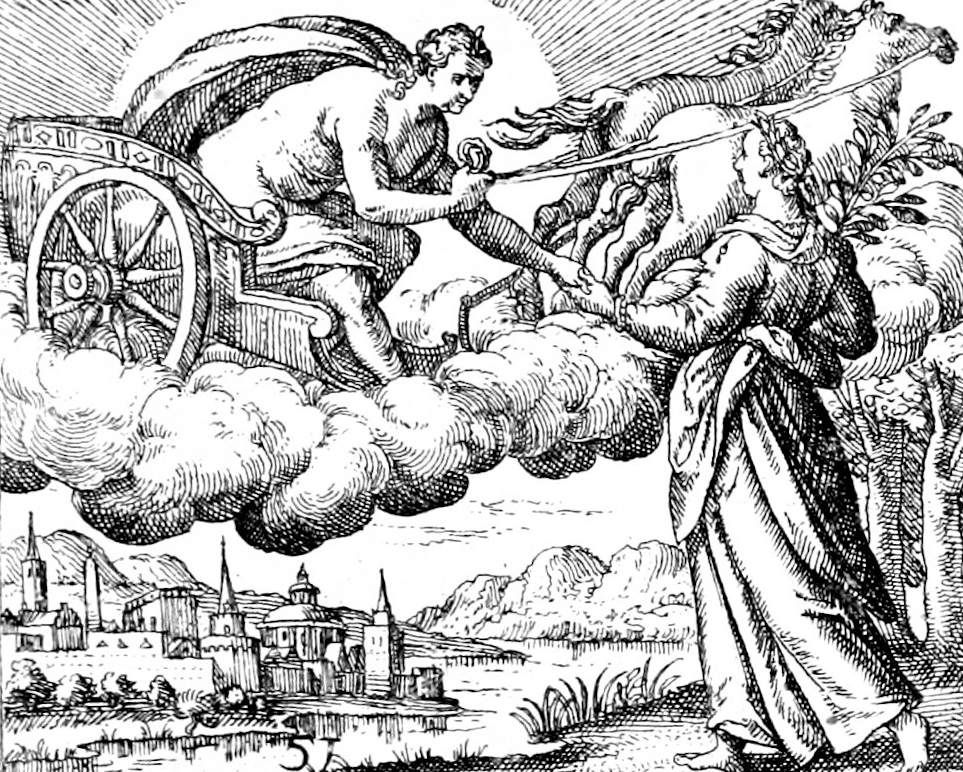
\includegraphics[width=1\textwidth]{images/brev14.png}
\end{center}

\breakpage